\chapter{Minimal Model}

In this chapter we will discuss the minimal model in depth. The minimal model, although it has only a few parameters and is quite simple in concept is able to explain a lot of the behaviour of Cas9. Furthermore, since it is the simplest model it is more intuitive and easier to pinpoint what exactly it does and does not do. Therefore it will function as a starting point for all our research.

\section{The first steps of the minimal model}

The first step in analyzing the minimal model is getting the correct values for the parameters in our model. The exact values of $\epsilon C, \epsilon I$ and $\epsilon PAM$ determine the behaviour of the model, therefore it is essential to get these values as accurate as possible. To obtain these values we will fit the model to data from \cite{PNAS}. This data set was chosen because it has several advantages over other data sets. For one it is very large, it contains all single and double mismatch and on top of that also sequences with more than two mismatches. Furthermore the authors have measured several properties of the enzymes: the on-rate, the off-rate and the occupancy. This allows us to fit on multiple data sets and test our fit for a different experiment.

\subsection{Methods of \cite{PNAS}}
\label{sec:BoyleMethods}

To better understand why we did certain things in our fitting procedure it is useful to understand how \citep{PNAS} performed their measurements. Firstly, \cite{PNAS} used a DNA sequencing chip over which they let flow a solution of dCas9. %TODO better name for chip
They knew exactly where each sequence was located on their chip. This allowed them to do fluorescence experiments and link the fluorescence signal to a specific sequence, by checking the location of the signal.

Secondly, it is good to note that all the experiments they performed were fluorescence experiments. This means all their experiments had all the issues that every fluorescence experiment has (calibration inaccuracies, diminishing signal, photobleaching, etc. [SOURCE]). For the occupation experiments the fluorescence is easily linked to the occupation of a certain sequence. If the signal is more intense then more of the enzymes are bound. If the light sensor is perfectly calibrated this allows you to directly link the fluorescence to the occupation. This is not as trivial for the effective on- and off-rates. These rates were also measured by linking the fluoresence to the occupation, but after this some fitting is necessary to extract the rate.

The effective on- and off-rates are measured by measuring the fluorescence signal at a 500 second interval and fitting a straight line through these points. The line is also forced to go through zero as, logically, at the start of the experiment none of the Cas9 is bound. To fit such a line using least-squares the following formula can be used: [SOURCE: $https://online.stat.psu.edu/~ajw13/stat501/SpecialTopics/Reg_thru_origin.pdf$ ]

\begin{equation}
\beta = \frac{\sum_i X_iY_i}{X_i^2},
\label{eq:slopeleastsquares}
\end{equation}

where $X_i$ is the x-value of the i-th data point and $Y_i$ is the y-value of the i-th data point. Solving this equation will give you $\beta$: the slope of the straight line which is fitted to the data. This line is forced to go through zero, so the offset $\alpha = 0$.

It is well-known and also logical that the this linear increase in occupation cannot hold for all times; a natural binding and unbinding process will follow an exponential which starts out as a linear process but eventually flattens gradually into an equilibrium, see figure \ref{fig:linearvexponentialexample}. The mathematical justification for the linear approximation is provided in section \ref{sec:mathematicaljustificationlinearapprox}. It will turn out this approximation is only valid for very fast times compared to the rates of the system.


\begin{figure}
\begin{center}
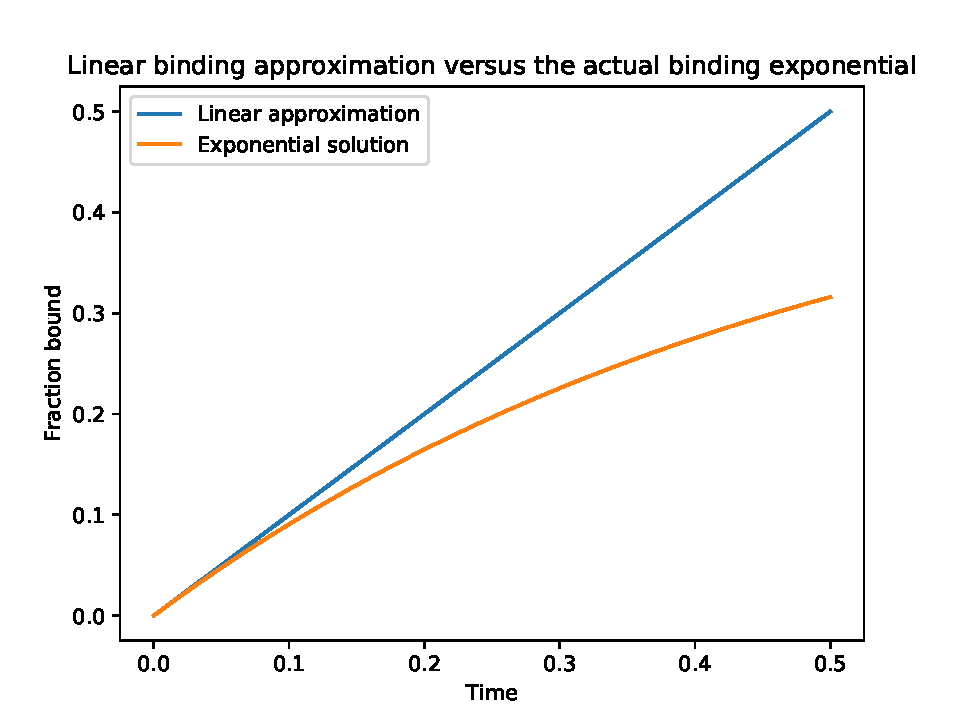
\includegraphics[width=\textwidth]{images/linearvexponentialexample}
\label{fig:linearvexponentialexample}
\caption{The difference over time between the bound fraction predicted by the linear approximation and the exponential solution. }
\end{center}
\end{figure}

\subsubsection{The linear approximation}
\label{sec:mathematicaljustificationlinearapprox}

In this section a brief justification of the linear approximation to the exponential binding curve of dCas9 will be given. Consider the system as described in the time-dependent section of the theory chapter (section \ref{sec:TimeDepTheory}). This describes the entire system for all times, but if we are only looking at the system for the very early times then no dCas9 will have made it to the end of this system. We can conclude that some of the states in our system can be ignored as they will have no effect on these short timescales. We can say that \textbf{if} we can approximate the unbinding of dCas9 as a single exponential, with a single rate, \textbf{then} we can model the system as a two-state system: one unbound and one bound state.

For the very short timescales it is easily justifiable that we can model the system with only one unbound and one bound state. All dCas9 is unbound at the start and after some average time the PAM is bound to the DNA. If the measurement stops before any dCas9 has the oppertunity to move on to the first bound state then the solution and the PAM state are naturally all the occupied states in our system. For slightly longer times where dCas9 has the time to form an R-loop it is still possible that the two-state approximation holds, as long as the bound states together behave as a single buond state, meaning they can be modelled as one state with a single dissociation rate, which must necessarily be different for every sequence.

The model has now simplified to the one in figure \ref{fig:two-state-model}. We can solve this simplified model with the master equation in the same way as in section \ref{sec:TimeDepTheory}. However, since this system only has two states instead of numerically it is possible to solve it analytically too.

First of all the total probablity to be either unbound or bound is one:

\begin{equation}
P_{bound}(t) + P_{unbound}(t) = 1.
\label{eq:sumPboundPunbound}
\end{equation}

Furthermore we know the time differential equations, since they are dictated by the rates:

\begin{align}
\frac{dP_{bound}(t)}{dt} &= k_f \cdot P_{unbound}(t) - k_b \cdot P_{bound}(t), \\
\frac{dP_{unbound}(t)}{dt} &= - k_f \cdot P_{unbound}(t) + k_b \cdot P_{bound}(t),
\end{align}

rewriting the top one using equation \ref{eq:sumPboundPunbound} gives:

\begin{align}
\frac{dP_{bound}(t)}{dt} &= k_f \cdot (1-P_{bound}(t)) - k_b \cdot P_{bound}(t), \\
\frac{dP_{bound}(t)}{dt} &= k_f - (k_f + k_b) \cdot P_{bound}(t).
\end{align}

Solving this gives the solution for both $P_{bound}(t)$ and $P_{unbound}(t)$:

\begin{equation}
P_{bound}(t) = c_1 \cdot \exp(-(k_f + k_b)t) + \frac{k_f}{k_f+k_b},
\end{equation}

which is easily solved by substituting the initial condition for $t=0$ to obtain the constant $c_1$. If we choose to start with all dCas9 in the unbound state we retrieve the exponential in figure \ref{fig:linearvexponentialexample} for the occupation of the bound state.

So this two-state approximation lets us analytically solve the master equation and model the total exponential. To get the linear approximation we need to go one step further. We can do a taylor expansion around $t=0$ for the occupation of the bound state to get:

\begin{equation}
P_{bound}(t) = (c_1 + \frac{k_f}{k_f+k_b}) + (c_1 \cdot -(k_f + k_b))t + \frac{1}{2}(c_1 \cdot (k_f + k_b)^2)t^2 + ...,
\label{eq:TaylorExpPB}
\end{equation}

if we then ignore terms of second order or higher and plug in the initial condition that $P_{bound}(t=0) = 0$, we obtain the linear equation:

\begin{equation}
P_{bound}(t) \approx (c_1 \cdot -(k_f + k_b))t = k_f \cdot t.
\label{eq:EffKFApprox}
\end{equation}

Here $c_1 = \frac{-k_f}{k_f+k_b}$ because $P_{bound}(t=0) = 0$. Equation \ref{eq:EffKFApprox} is the approximation used to calculate the effective forward rate in the experiments of \cite{PNAS}. Note that we have used two approximations to obtain this result:

\begin{itemize}
\item The system can be approximated by only two states: one bound state and one unbound state. This approximation is valid only if the unbinding can be approximated by a single exponential unbinding curve with a single unbinding rate.
\item We can neglect all second order and higher terms in the Taylor expansion of equation \ref{eq:TaylorExpPB}. This is valid only if $\frac{(k_f+k_b)t}{2} \ll 1$.
\end{itemize}

\begin{figure}[H]
\begin{center}
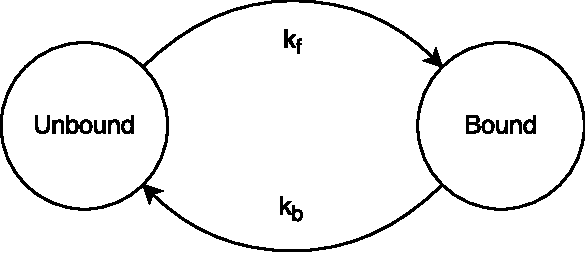
\includegraphics[width=\textwidth]{images/TwoState}
\label{fig:two-state-model}
\caption{A schematic representation of the simplified two state system.}
\end{center}
\end{figure}
 


\subsection{Observations from \cite{PNAS}}

In the previous section we have reiterated how \cite{PNAS} performed their measurements, In this section we will take a look at their observations by primarily examining the three heatmaps they have provided: figures 2B, 3A and S2 in \cite{PNAS}.
These heatmaps show the effective on-rate, the effective off-rate and the occupation in equilibrium respectively. If the minimal model is to hold then it has to be able to explain the observations that are made in these heatmaps. Since the minimal model is as simplistic as possible it is unlikely that it is able to explain every feature in the data, however assuming that the general underlying model is correct, even the minimal model should be able to qualitatively describe most of the features found in the data. Let us first take a look at the effective on-rate.

\subsubsection{Effective on-rate}

First of all note that there is a sequence dependent effective on-rate at all. This does not comply with the requirements for the linear approximation we have established at the end of section \ref{sec:mathematicaljustificationlinearapprox}. Specifically the second requirement $\left( \frac{(k_f+k_b)t}{2} \ll 1 \right)$ does not hold, since evidently equation \ref{eq:EffKFApprox} does not hold. Therefore we are not in the purely linear, and therefore sequence independent, regime. Since the sequence can only alter the backward rate from the bound state there must be at least some influence of higher order terms. The second order term is:

\begin{equation}
\frac{-k_f}{2} \cdot (k_f+k_b)t^2.
\end{equation}

Here we see that the influence of the backward rate is to decrease the amount of bound dCas9, as expected. Sequences with closer mismatches have to cross the mismatch sooner than sequences with later mismatches. Therefore they run into a barrier sooner and have to backtrack only a few steps to unbind, in contrast with the sequences which have a terminal mismatch. These terminal mismatch sequences have to backtrack almost the entire R-loop to unbind and are therefore less likely to unbind before making it over the mismatch barrier. Consequently the earlier the mismatch the higher we can approximate the backward rate from this single bound state. From \cite{Misha} we know that the probability to make it past the mismatch before unbinding follows a sigmoidal curve. If we assume it is almost impossible to unbind once a dCas9 has made it past the mismatch it is logical that the backward rate $k_b$ also follows a sigoidal curve, but inverted (starting high and ending low). Therefore the minimal model would also, very generally, predict a sigmoidal curve (from low to high) for the effective on-rate.

\subsubsection{Effective off-rate}

The analysis for the effective off-rate is made more complicated since the initial condition is not as simple as the one for the effective on-rate. The initial condition for the dissociation experiment is the equilibrium of the system. This equilibrium can easily be calculated using boltzmann factors as explained in section \ref{seq:EquilTheory}. It is hard to justify taking all these different bound states together and collpasing them into one single bound state, since the argument that only very little time has passed and the last states do no contribute anything does not hold anymore. If we simply ignore these issues for now we can at least try to compare the data to the simplified two-state model.

\cite{PNAS} make a remarkable discovery in their dissociation experiment: the existence of a special, unstable region between the seed region and the terminal bases. They name this region the reversibility determining region (RDR). This special region is characterized by an increased dissociation rate compared to the seed region when a the first mismatch of the sequence is placed in this region. In other words: the most unstable R-loop is formed when the first mismatch of a sequence is placed in the RDR.

This observation is not in agreement with the minimal model. We have established that the dissociation rate from the bound state is higher is the mismatch is at the beginning of the DNA sequence and gets lower as the mismatch is moved to the end. Therefore one would expect that the effective off-rate that is measured also decreases as the mismatch is moved towards the end of the DNA sequence. Note that the simplified two-state system can never explain both the effective on-rate and effective off-rate ersults from \cite{PNAS}. If the actual on-rate is the same for all sequences then the difference in effective on-rate between sequences must stem from a difference in dissociation rate. This assumption is easily justified in the zipper model as the unbound dCas9 enzyme has no knowledge of the sequence beyond its interaction with the PAM.

The RDR is even more problematic than that as, even if we include all possible bound states, the minimal model always predicts that, the closer the mismatch, the more unstable the entire R-loop is. Therefore the dissociation results are harder to explain than the association results.


\subsubsection{Occupation}

The final heatmap that is published in \cite{PNAS} is supplementary figure S2.
Here the authors show the intensity of the fluorescence signal after twelve hours. For the purposes of this report it is assumed that the mixture of DNA and dCas9 is in local equilibrium after twelve hours. It is hard to justify this assumption definitively, but we will try to make it at least believable.

First of all, in order to function as an effective immune system for the bacteria who use CRISPR as a means to fend off virusses it is necessary that Cas9 is able to cleave the correct sequences quite quickly. If Cas9 is able to cleave the on-target then it must have reached the fully bound R-loop state. It is then a reasonable assumption that the on-target is able to reach equilibrium after twelve hours. Of course, adding mismatches slows down the entire binding process. However it is also known that Cas9 is able to cleave invasive virus RNA containing a mismatch as a means of defending itself. Therefore the mismatch barrier cannot be insurmountable on these, relatively short, timescales. It is then not far-fetched to also assume that double mismatches could be overcome in twelve hours. %TODO binding times source!

Secondly, we assume that the system is in a local equilibrium, instead of a global equilibrium. This means that the individual clusters on the DNA sequencing chip are in equilibirum with their immediate surroundings, but the entire chip is not in equilibrium. %TODO better name for sequencing chip.
This is harder to justify than the claim that the chip is likely in equilibrium. One argument is that, if the entire chip was in equilibrium, all double mismatch sequences would be outcompeted almost entirely by the on-target sequence. This is not what happens in the experiment and therefore it is unlikely that the entire chip is in global equilibrium. This argument ignores the effect of competition between sequences and assumes there is an infinite amount of on-target sequences (and all other sequences) to bind to, which is obviously not the case on the actual chip. Nevertheless one might expect a more skewed image, with much more fluorescence concentrated at the on-target and single mismatch sequences, if the chip was in a global equilibrium. A second argument in favor of a local equilibrium instead of a global equilibrium is that to establish a global equilibrium every dCas9 enzyme must have had the oppertunity to explore the entire chip and all available states. The diffusion coefficient of a small protein in water is about $100 \mu m^2/s$ \citep{brune1993predicting}.
This means in twelve hours every protein has had the ability to explore $4.32 mm^2$ of the chip. However while diffusing dCas9 also binds and unbinds to the DNA sequences it encounters, so this estimation is necessarily an overestimation. Since this explored surface area is on the same order of magnitude as that of the chip, combined with the fact our calculation is an upper limit it is not unreasonable to say that not every dCas9 has the oppertunity to explore all the available states. %TODO chip size.

The general zipper model is able to predict the fraction of bound dCas9 by calculating the boltzmann weight of every available state. Using these weights it is possible to calculate the probability to be in any state, given that the system is in equilibrium, as described in section \ref{sec:EquilTheory}. The minimal model merely provides a way to prescribe the energy of each state so the boltzmann weights can be calculated. The minimal model predicts that the further down the mismatch, the more stable the R-loop and therefore a larger fraction of bound dCas9. It also predicts an interaction between mismatches which form a region analogous to the $n_{pair}$ region from \cite{Misha}. Both these observations can be seen in the occupation heatmap from \cite{PNAS}, albeit that the seed region is much more pronounced than the $n_{pair}$ region. This can however simply be a matter of parameter values.


\subsection{Initial expectation of the minimal model}

So far we have taken a closer look at how \cite{PNAS} measured their data and some of the conclusion they have drawn from that. We established that the minimal model is likely able to predict similar features as the ones shown in the association data and the occupation data. However the RDR in the dissociation data is not predicted at all by the minimal model. Furthermore we have established that the association and dissociation data cannot simultaneously be explained by a simply two-state model. In the next section the minimal model will be put to the test and we will attempt to reproduce the results from \cite{PNAS} using the minimal model, starting with the occupation data.



\section{Occupation fit}

Since we expect the effective on-rate data and the occupation data to be more easily explained by the minimal model than the dissociation data and the occupation data contains two parameters less, the first fits will be on the occupation data from the supplementary information in \cite{PNAS}. %TODO figure numbers? - should I put their figures in my thesis?
For the fitting of the minimal model to the occupation data the simulated annealing algorithm, described in chapter \ref{ch:SA} is used.

\subsection{Model for the fit}
To fit the minimal model to the occupation data the model explained in section \ref{seq:EquilTheory} is used. The minimal model assigns a specific energy to each state in the model based on whether the base pairs match and every match or mismatch before. With these energies it is possible to calculate the equilibrium distribution of dCas9 over all available states with the Boltzmann weights. It is therefore possible to calculate the probability to be bound given any sequence.

\subsection{Data for the fit}
The provided occupation data from \cite{PNAS} contained the fluorescence intensity of single sequences before association and before dissociation. Of course the fluorescence intensity is linked to the amount of bound dCas9, however the nature of fluorescence necessitates some form of normalization before the measured intensity reflects the actual fraction of bound dCas9. Furthermore it is helpful to be aware of the fact that there is a non-negligible amount of noise in the measurements. %TODO justify.
To circumvent these issues with the data, the data was transformed before the fit. First the pre-association intensity was subtracted from the pre-dissociation value for each data point separately. Since before any association no dCas9 should be bound the pre-association intensity value is attributed to noise. After this the median intensity was calculated for every sequence. Since the variance in each sequence is quite large, taking the median and fitting to that will most likely produce better results as the noise is reduced, assuming the noise is symmetric. Finally the median intensity value for each sequence is divided by the median intensity value for the corresponding on-target sequence. This allows us to see how much each sequence binds compared to the on-target sequence. This ratio is no longer in arbitrary units; no matter the units the ratio is the same. Another advantage of this ratio is that it makes the results easier to interpret. The on-target should, logically, bind the most out of any sequence so every mismatched sequence should result in a ratio of less than $1$ and the closer to $1$, the less impact the mismatch has had on the binding.


\subsection{Fit results}
\label{sec:minmodelresults}

%TODO include spearman coefficient or some other form of comparison tool

The fit was performed nultiple times on replica 1 and replica 2 from \cite{PNAS} separately. Furthermore the fit was also repeated several times on different subsets of data. This allows for testing of the model within the total data set as well as testing on other data sets. We will start by showing the fit on the total data for replicas one and two separately; these results can be found in figures \ref{fig:MinModelResultsHM} and tables \ref{tab:MinModelResultsRep1} \& \ref{tab:MinModelResultsRep2}. %TODO reference figures and table of results


\begin{table}
\begin{center}
\csvautobooktabular{tables/Rep1MinModelResults.csv}
\caption{Table containing the fit results for the energy gain of a match, the energy penalty of a mismatch and the energy penalty of the PAMfor replica one. The average of the fit results is reported in the bottom row. When calculating the average, fit \# 4 is omitted since it is an outlier.}
\label{tab:MinModelResultsRep1}
\end{center}
\end{table}

\begin{table}
\begin{center}
\csvautobooktabular{tables/Rep2MinModelResults.csv}
\caption{Table containing the fit results for the energy gain of a match, the energy penalty of a mismatch and the energy penalty of the PAM for replica two. The average of the fit results is reported in the bottom row. When calculating the average, fits \# 5 and \# 6 were omitted since they are outliers. Note that there is one less fit result than for replica 1 as one of the fits failed to produce any results. }
\label{tab:MinModelResultsRep2}
\end{center}
\end{table}

\begin{figure}
\begin{center}
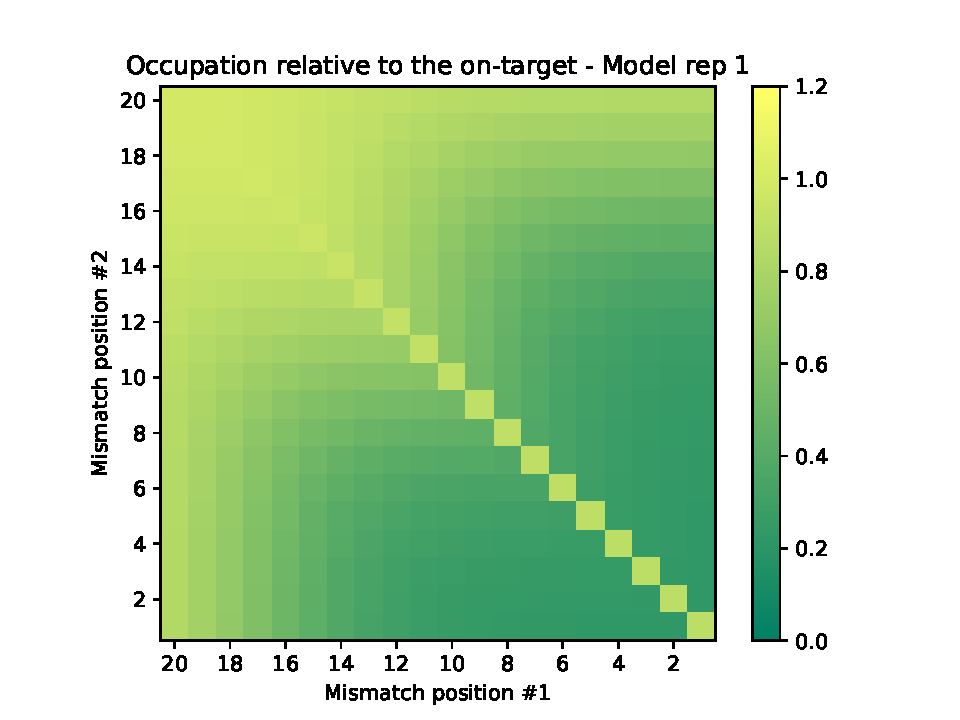
\includegraphics[width=0.45\textwidth]{images/MinModelRep1}
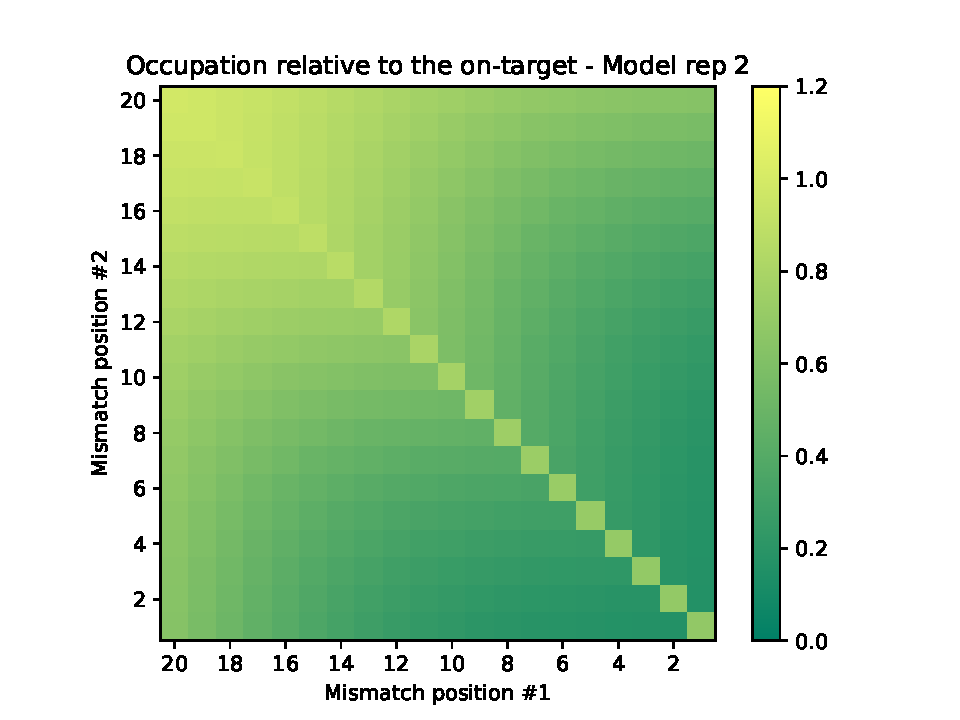
\includegraphics[width=0.45\textwidth]{images/MinModelRep2}
\caption{These heatmaps show the predicted occupation in equilibrium based on the minimal model with parameters that were obtained from fitting to replica 1 (left) and replica 2 (right) from \cite{PNAS}. The average values from tables \ref{tab:MinModelResultsRep1} and \ref{tab:MinModelResultsRep2} were used for these heatmaps. On the diagonals the single mismatch predictions are shown. }
\label{fig:MinModelResultsHM}
\end{center}
\end{figure}

Figures \ref{fig:MinModelRep1ErrorsHM} and \ref{fig:MinModelRep2ErrorsHM} %TODO reference figures with errors
may be even more useful. They show the relative and absolute error in the prediction. When examining these errors it is important to realize that the fitting function that was used to obtain the model parameters minimizes the \textit{absolute} error, not the relative error.

\begin{figure}
\begin{center}
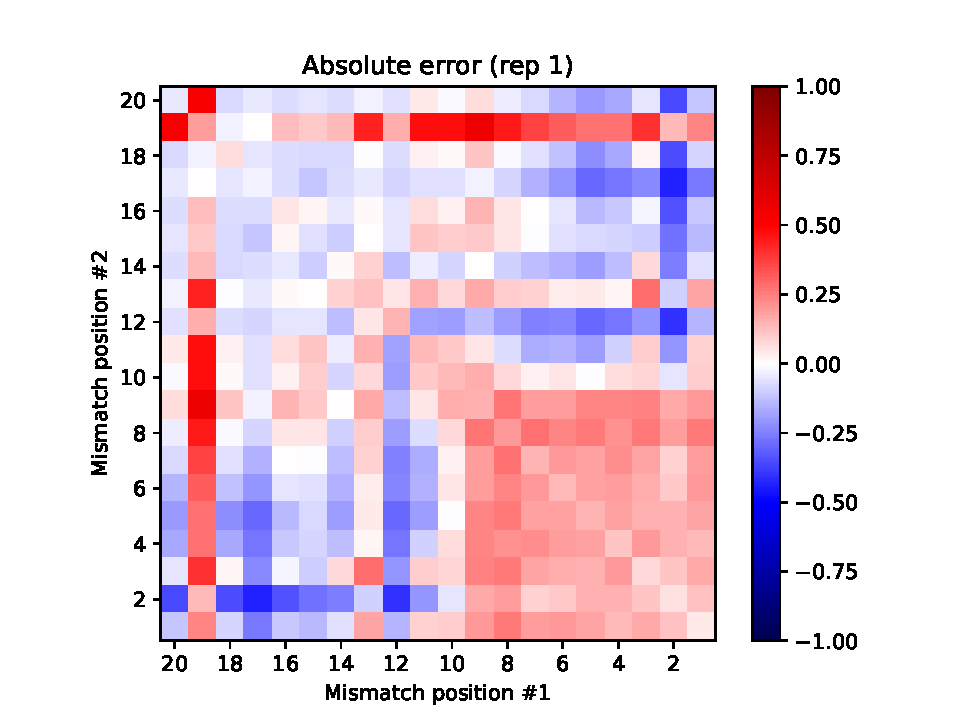
\includegraphics[width=0.45\textwidth]{images/MinModelRep1AbsErr}
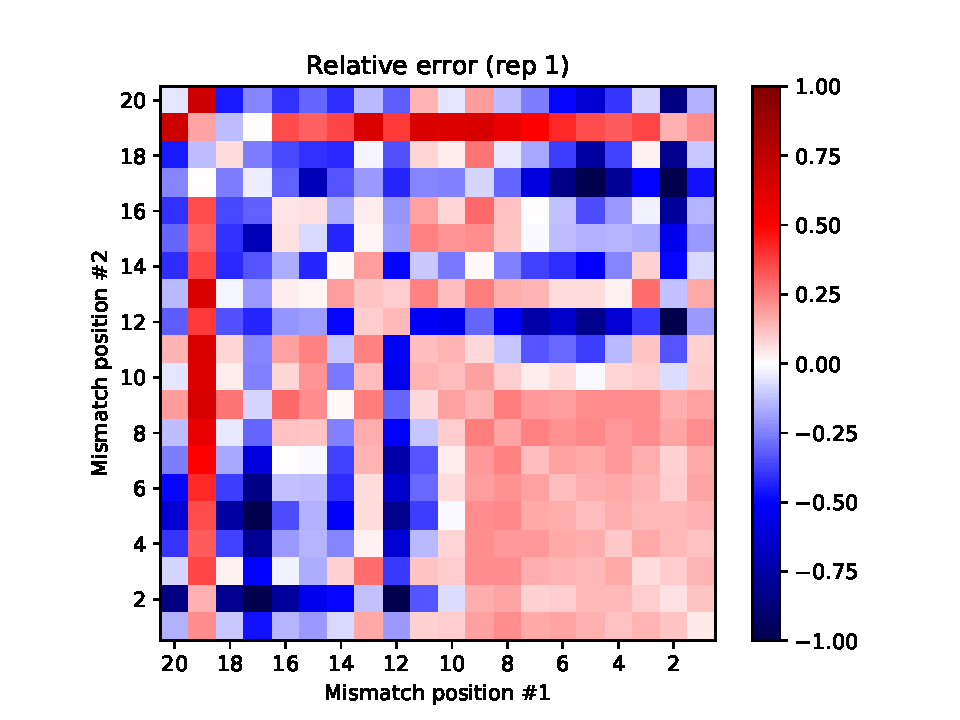
\includegraphics[width=0.45\textwidth]{images/MinModelRep1RelErr}
\caption{These heatmaps show the absolute difference between the measured and the predicted occupation in equilibrium based on the minimal model. Both the measurement and the fit were done on replica 1 from \cite{PNAS}.}
\label{fig:MinModelRep1ErrorsHM}
\end{center}
\end{figure}

\begin{figure}
\begin{center}
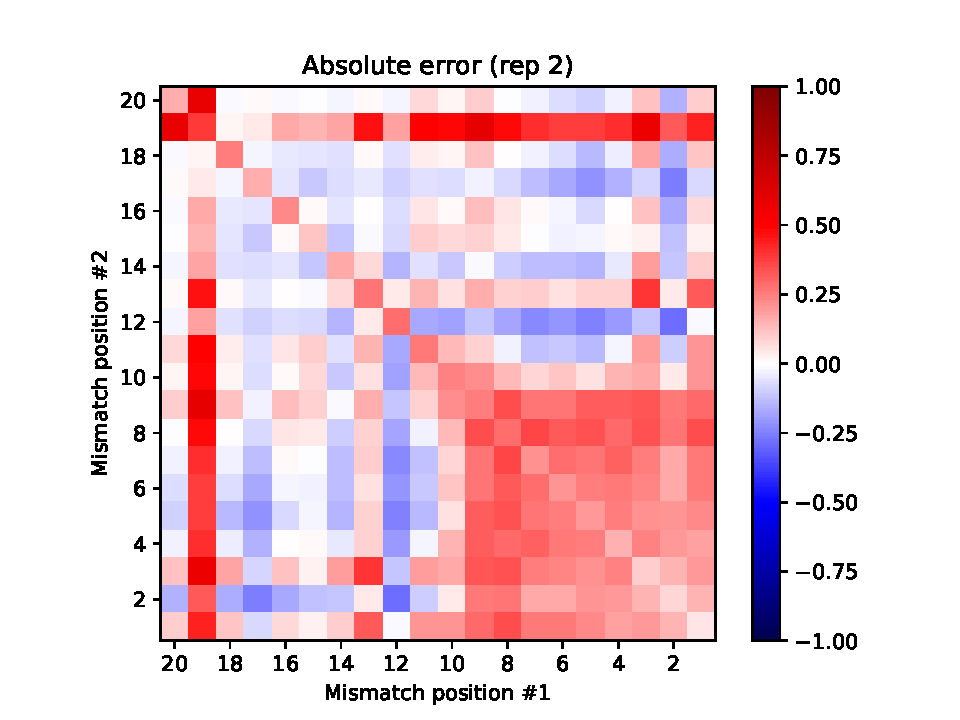
\includegraphics[width=0.45\textwidth]{images/MinModelRep2AbsErr}
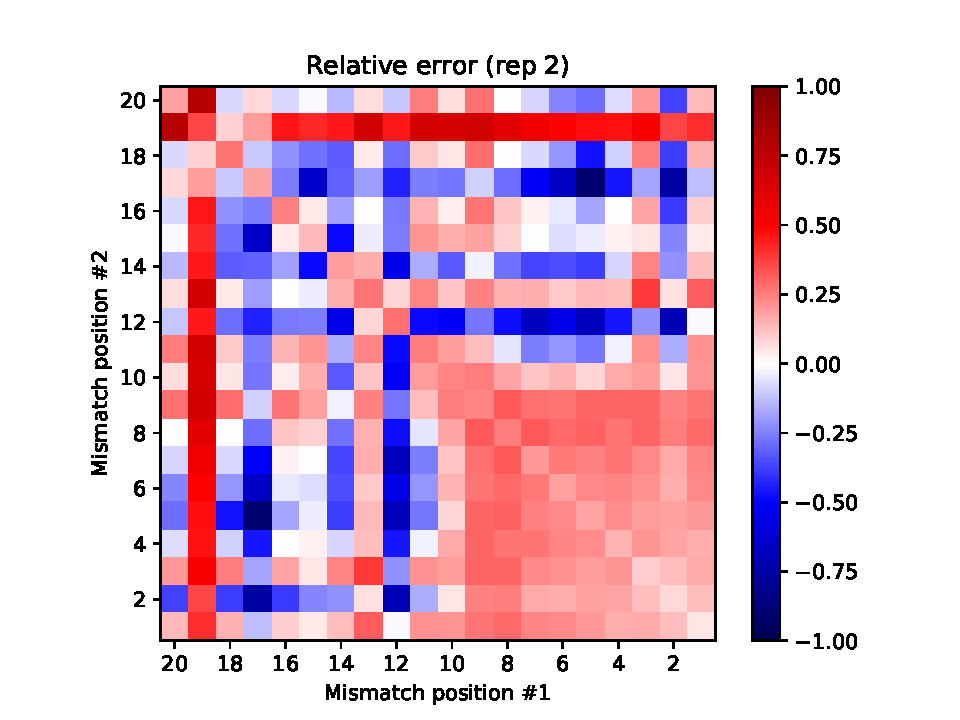
\includegraphics[width=0.45\textwidth]{images/MinModelRep2RelErr}
\caption{These heatmaps show the absolute difference between the measured and the predicted occupation in equilibrium based on the minimal model. Both the measurement and the fit were done on replica 2 from \cite{PNAS}.}
\label{fig:MinModelRep2ErrorsHM}
\end{center}
\end{figure}


Several specific features of these results will be looked at in greater detail in following sections. One surprising result we would like to bring to your attention now however is the positive value for the PAM energy. It turns out that the best fit to the data is one where binding to the PAM is unfavorable compared to the solution state. This is allowed within the minimal (and general) model as it violates no assumption that was made in section \ref{seq:generalmodel}. It was mentioned that a matching PAM sequence should be favorable compared to a non-matching PAM sequence. Since this can still be the case a positive $\epsilon PAM$ is allowed within the model. In section ... %TODO ref section
it is also explained that the PAM, and therefore all energies, are concentration dependent. Thus the actual PAM energy in-vivo could possibly be much lower. %TODO back-of-the-envelope calculation..

Note that we have not allowed for a positive $\epsilon C$. While one could argue that a match should merely be favorable compared to a mismatch and is not necessarily an absolute energy decrease, we would like to justify our assumption by reminding people of the origins of Cas9. Cas9 is naturally used to protect bacteria against viruses. If a match would be an absolute energy increase, it would be unlikely or take long to cleave any target, including the on-target. Therefore Cas9 would not be very effective as an immune system if a match would be an absolute energy increase. Finally one could also argue that there is an energy increase but it is tiny. If that was the case however the fitting algorithm would most likely have found a very low decrease in energy to match the reality as well as possible. Since the optimal parameters are not near zero it is probable that a match is an energy decrease. 

%TODO perhaps move most of this section to the theory section on the minimal model... <<<<<
\subsubsection{Seed region}
\label{sec:minmodelresultsseedregion}

In the fit the seed region corresponds to the seed region in the data. In both experiment and theory the shift from a low to a high occupation occurs around base pair ten. In the theory this is very naturally explained by the fact that around base pair ten the energy of the formed R-loop dips below the energy of the solution. This is illustrated in figure \ref{}... %TODO

%TODO illustrate seed region

Figure \ref{}.. %TODO same figure as before
provides a nice geometric and intuitive way to see the transition from the low occupation to the high occupation. It is also possible to make some simplifications and calculate the approximate gain in occupation for each subsequent matching base. It is known that in equilibrium the occupation of each state is given by

\begin{equation}
P(s) = \frac{\exp(-E_s)}{\sum_{s=-1}^{s=20}\exp(-E_s)},
\end{equation}

where $s$ is the state, numbered $-1$ to $20$ in this case. The ratio between the occupation of two states is

\begin{equation}
\frac{P(a)}{P(b)} = \frac{\exp(-E_a)}{\exp(-E_b)}.
\end{equation}

If we assume that the energy gain for a match is large and that $a$ and $b$ are subsequent states ($b = a+1$), which are both matches, then the ratio of the occupancy becomes:

\begin{equation}
\frac{P(a)}{P(b)} = \frac{\exp(-E_a)}{\exp(-(E_a + \epsilon C)} = \frac{1}{\exp(-\epsilon C)} = \exp(\epsilon C) \approx 0,
\end{equation}

where the last approximation is made since $\epsilon C$ is large and negative. In this case all dCas9 would occupy state b instead of state a, we will call state b the dominant state.

If we assert, on top of the assumption that $\epsilon C$ is large, that the first mismatch in a sequence occurs at position $n+1$ then there will be two dominant states competing for the dCas9: the solution state and state $n$. This is because $\epsilon PAM$ is positive, allowing the solution state to be the dominant state even though the PAM and the first $n$ base pairs matched. The ratio between the two dominant states is then:

\begin{equation}
\frac{P(-1)}{P(n)} = \frac{1}{\exp(-E_n)} = \exp(E_n),
\end{equation}

so with these assumptions the ratio of unbound to bound decreases exponentially as the first mismatch gets pushed back further, since $E_n$ becomes lower and lower. More exactly: if the mismatch is pushed back one base pair then the ratio of the unbound to the bound fraction decreases with a factor $\exp(\epsilon C)$. %TODO See how well this matches the model and maybe even the data?
This also proves that, as the geometric insight already implied, once the energy dips below the energy of the solution state the occupation rapidly increases, which marks the end of the seed region.


\subsubsection{Stripes}

A significant difference between the prediction of the minimal model and the experimental results are several 'stripes'. These features are rows and columns in the occupation heatmap for which the minimal model predicts a low occupation, while a high occupation is measured by \cite{PNAS}. Less pronounced are also the opposite stripes, where the model predicts a high occupation while the experiment measures a low occupation. These features undoubtedly exist within the data but can never be predicted by the minimal model. The minimal model does not allow for an increase in occupation followed by a decrease in occupation or vice versa; the minimal model is monotonic. The reason for this is two-fold. Firstly, every match or mismatch affects the energy of all subsequent states. This is however true for all models that fall within the general zipper model described in chapter \ref{ch:Theory}. The reason the minimal model is monotonic is because the minimal model only has one single parameter for a match and another single parameter for a mismatch. Therefore the minimal model can not contain any local effects. Coupled with the first point the minimal model is necessarily monotonically increasing in occupation versus the first mismatch position.

The stripes visible in the data thus point towards some very fundamental properties of the energy landscape which determines the binding of dCas9. There need to be some local and/or neighbor effects incorporated into the model to better predict the results from \cite{PNAS}. These stripes, especially the one where a mismatch occurs at position two, also show up in different data sets. %TODO cite Pattanayak?

A simple addition to the model could be a position dependent $\epsilon I$. For example, if the $\epsilon I$ at position two is much lower than other $\epsilon I$, a mismatch at position two would prohibit binding much less than mismatches at other positions, resulting in a higher occupancy. This is a simple addition to explain a single striped pattern. There are other models that would be able to explain this striped pattern, we merely bring up the position dependent model to show the stripes could be explained by a more complicated energy landscape.


\subsubsection{Upper plateau}

A third feature that is apparent in the data but not in the model is hidden in the region where the occupancy is highest. In this region the model predicts an occupancy of almost $1$, meaning the same occupancy as the on-target. This is a logical prediction within the minimal model as a double mismatch at positions nineteen and twenty would still have $18$ matching base pairs before any mismatches occur. If the seed region extends to base pair ten then ten matching base pairs approximately bring the energy of the R-loop down to the energy of the solution, resulting in about an even split between bound and unbound dCas9, as we have seen in section \ref{sec:minmodelresultsseedregion}. If another eight matching bases are then added beyond the seed region the bound fraction is approximately $0.5 \cdot \exp(-8\epsilon C)$, which approximately equals $1$ if $|\epsilon C|$ is not absurdly low.

The model is quite clear with its results in this high occupancy region, but the data is not so clear. According to the data these sequences with mismatches at the final few bases are actually easier to bind to than the on-target; resulting in measured occupancies higher than $1$. This is strange behavior when you consider the original role of Cas9 in the immune system of a bacterium. Logically one would say that Cas9 would be best at cleaving the on-target sequence, as that is the sequence which corresponds exactly to the gRNA. This property would also make it perform best at defending against invading viruses which match the gRNA sequence. Of course it could be that these sequences are more favorable to bind than the on-target sequence but it would contradict some of the assumptions we have made at the very start for the general zipper model. These abnormally high occupancies could be explained be an (position dependent) energy penalty for a match or a (position dependent) energy gain for a mismatch. However other models which would not contradict the general assumptions so blatantly could perhaps also explain this behavior. Effects from neighboring bases, sequence related effects or protein related effects can all also be causes for the increased occupancy of these off-targets. Finally, although the data quality is good, %TODO prove?
the increased occupancy measurements could also simple be the result of noise. If the noise is relative to the signal strength then this would explain why this effect is less apparent in the low occupancy region. However the increased occupancy seems to be consistent throughout the entire high occupancy region, which is not what you would expect if the effect was purely caused by symmetric noise.

\subsubsection{Pair region}
At the very edges of the heatmaps there are again regions with a higher occupation even though they contain mismatches within the seed. These regions are the pair regions where the mismatches interact in such a way that there can still be significant binding even though there is a mismatch early in the sequence. This 'second seed region' effect is described in \ref{sec:TheoryPair}. For some sequences it can easily be understood; for example a sequence with mismatches at positions one and twenty. This sequence essentially behaves as a sequence with only a single mismatch at position one, since the mismatch at position twenty has a negligible effect on the binding. For other sequences it is less clear and size of the pair region is actually determined by the ratio of mismatch energy penalty to match energy gain. In the case of the minimal model for replica one this ratio is approximately $6.16$. Therefore the pair region should be another six to seven bases after the seed region. For replica two the pair region is another eight to nine bases after the seed. Both these numbers can be confirmed if we take a look at figure \ref{fig:MinModelResultsHM}. On the left (replica one) we see a seed region of ten to eleven basepairs, as confirmed by the fit, and the pair region shows up around basepair seventeen. On the right (replica two) we see a seed region of around fourteen basepairs and the pair region is therefore much less pronounced. It is still possible to see the very start of the pair region since the match gain is quite low, so transitions are stretched out over many basepairs.


\section{Effective on-rate fit}

Fitting to the occupation data fixed all energies in the minimal model. Knowing these three parameters allows you to predict the equilibrium state of the system, however to predict the time evolution of the system more parameters need to be known, as discussed in section \ref{sec:TimeDepTheory}. These parameters are the 'on-rate' and the 'attempt rate' of the system: the rate of binding from solution to PAM and the rate of moving from any bound state to any other state respectively. In this section these two parameters will be fit to the effective on-rate data gathered by \cite{PNAS}.


\subsection{Model for the fit}
The model that is used will be based on the master equation which is described in section \ref{seq:TheoryTimeDep}. To be able to fit the model to the data from \cite{PNAS} it is necessary to model the experiment as accurately as possible. The details of the experiment are repeated in section \ref{sec:DetailsDataOnRate}. To model the experiment as accurately as possible we followed the procedure:

\begin{enumerate}
\item Nothing is bound at the start of the experiment.
\item The occupancy is calculated at three evenly spaced timepoints.
\item The bound fraction at each timepoint is calculated by summing over the occupancy of each state except the solution state.
\item A straight line is fitted through the bound fraction values. This line is forced to go through $(0,0)$.
\item The slope of the fitted line is the effective on-rate.
\end{enumerate}

This is the procedure followed by the experiment translated to the minimal, time-dependent, model. Of course in the experiment step two and three are simply replaced by measuring the intensity, which should be equal to the occupancy of the bound states up to some constant factor and noise.

The general procedure is clear, however some details of the model still need to be determined. We will go through the general procedure step by step and see what each statement means for the calculation. The first step is that nothing is bound at the start of the experiment, you start off clean. This is easily translated to the model, where it is possible to simply intialize the occupation vector with all of dCas9 in the unbound state. The occupation vector in this context is the vector which contains the occupancy of each state. Assuming the first state of the occupation vector is the solution state we initialize the vector as:

\begin{equation}
\vec{P}(t=0) = \left[ 1, 0, 0, 0, ..., 0, 0 \right].
\end{equation}

The second step of the general procedure is to calculated the occupancy of each state at three evenly spaced timepoints. Within this step essentially the entire minimal model is hidden. To calculate the occupancy at different timepoints two things are needed: the occupancy of each state at a single timepoint, the initial condition, and the rate matrix, which describes the evolution of the occupancy vector through time. If these two things are known it is possible to evaluate equation \ref{...} at any timepoint. Luckily the initial condition is known from the previous step. The rate matrix is not entirely known, it depends on both the energy landscape and the rates from the minimal model. In this fit the energy landscape is fixed from the occupancy fit, however the rates are still free. The rates are therefore the parameters that will be fitted. In the minimal model we will make the assumption that all attempt rates are equal as described and justified in section \ref{sec:TheoryTimeDep}. This reduces the number of rates that need to be fitted to only two. Knowing the energy landscape and the fitted rates allows us to calculate the occupancy at the three different timepoints and move on to step three. Step three, four and five are all relatively straightforward. The occupancies that are calculated in step two will be used to calculate the bound fraction of dCas9. In this case again it is assumed that dCas9 is bound when it is not in the solution state. In step four a line is fitted to the occupancies, this fitting procedure is described in section \ref{sec:BoyleMethods} and is the same fitting procedure as is carried out by \cite{PNAS}. Finally in step five the effective on-rate is obtained from the model which can be compared to the measured effective on-rate. 

%TODO Switch Model and Data sections around for more fluid story..? - Feels double now and confusing now.
\subsection{Data for the fit}
\label{sec:DetailsDataOnRate}
The provided effective on-rate data from \cite{PNAS} contains the slopes of the intensity curve for each sequence. To extract a slope of the fluorescence curve per sequence out of the fluorescence intensity for each single DNA strand the median fluorescence value per tile was taken. This was then normalized by the median fluorescence of the on-target after 12 hours of binding. After 12 hours of binding the on-target is expected to be fully bound and this is confirmed by the experiment. The median intensity value per tile is used to \textit{'account for systematic differences in focus, cluster formation efficiency and illumination across tiles'} \citep{PNAS}. The intensity values are then normalized by the on-target fluorescence in equilibrium to convert the intensity to an occupation. This normalization by the on-target intensity in equilibrium is absent in the minimal model that was used as the model is able to directly work with occupancies and has no need for any conversions. As long as the bound fraction of dCas9 for the on-target in equilibrium is approximately equal to one this is a justifiable omission and as confirmed in section \ref{sec:minmodelresults} this is indeed the case.

\subsection{Fit results}
The fit was performed on replica 1 and 2 from \citep{PNAS} separately and repeated several times. The results of the fit are more conclusive than the the results of the occupation fit, as can be seen in table \ref{...}. The fit results are shown as a heatmap in figures \ref{...} and \ref{...}. As with the occupancy fit the absolute and relative errors are also plotted in heatmap format in figures \ref{...} and \ref{...}. Again, these fits were performed with the simulated annealing algorithm described in chapter \ref{ch:SA} and minimize the absolute error.

%TODO
% Explain why On Rate does not matter.

%\begin{table}
%\begin{center}
%\csvautobooktabular{tables/Rep1MinModelResultsOnRate.csv}
%\caption{}
%\label{tab:MinModelResultsRep1}
%\end{center}
%\end{table}

%\begin{table}
%\begin{center}
%\csvautobooktabular{tables/Rep2MinModelResultsOnRate.csv}
%\caption{}
%\label{tab:MinModelResultsRep2}
%\end{center}
%\end{table}

%Heatmap with results
%Error heatmap

The effective on-rate results contain less features in their heatmap, for the data as well as for the fit. Some form of seed region can indeed be seen in the data and there is definitely some position dependence, on account of the striped pattern also present in the occupation fit. This position dependence is not contained within the minimal model. However it may be more interesting to discuss the features that are absent in this effective on-rate heatmap: the pair region where the two mismatches interact.

Note that the attempt rate between fits is really consistent but the on-rate is not. The reason for this becomes clear if we draw the $\chi^2$ landscapes for both parameters leaving one fixed (figures \ref{..} and \ref{..}). Both curves have the shape of a Lennart-Jones potential, however the flat part for the attempt rate is higher than its lowest point at the predicted attempt rate. For the on-rate the valley seems to be missing entirely and the sharp decrease at the start is simply followed by a flat line which extends far. This suggests that the on-rate simply needs to be large compared to the attempt rate in order to have a good fit; the actual value does not matter as much. This is also quite logical since the on-rate determines only two things: the rate at which dCas9 moves from solution to the PAM state and the probability to go from the PAM state to the first base pair state. Once the on-rate is large compared to the attempt rate these two effects cancel out. If the on-rate doubles the probability to go from PAM to first base pair is halved, but at the same time the time it takes to go from solution to PAM is also halved, meaning there are twice as many opportunities to move past the PAM state. This effect ensures that as long as the on-rate is large compared to the attempt rate its exact value does not matter as much.

\subsubsection{Seed region}
It is clear from section \ref{sec:minmodelresultsseedregion} why the occupation heatmap should show a seed region, however this does not explain why the effective on-rate map should also contain such a seed region. When out of equilibrium the binding to each sequence does not know how many states there are below the energy of the solution state down the line. The most important interaction of the system is the one of the binding base pair. The reason a seed region is still visible is therefore unlikely to be due to some global effects of the system. In other words the actual on-rate from solution to bound PAM is the same for every sequence with the same, matching, PAM. The reason a seed region is visible is because we are measuring the effective on-rate. The dCas9 has the time between measurements to move between several states. This allows dCas9 to bind to the sequence, go several base pairs in and make it across a mismatch barrier or be bounced back from the mismatch barrier. Essentially dCas9 has the time to, in between measurements, explore the energy landscape. This allows the enzyme to feel the interaction of more than the first few base pairs and can result in some form of seed region. To make it intuitive why this exploration of the energy landscape can lead to some form of seed region it might be informative to push some of the energy landscape parameters to the extreme. Consider the case where $\epsilon I = \inf$ and $\epsilon C \ll -1$. Here the PAM pushes the energy of several states up and the energy gets a lot lower whenever another match is added to the sequence. However when dCas9 encounters a mismatch it is impossible to make it over the mismatch energy barrier. The enzyme has only one choice: to unbind again. Assume now that the attempt rate is fast $k_0 \gg 1$, then once an enzyme is bound it quickly moves down the sequence until it encounters a mismatch. When it does it will move between the bound states and unbind eventually. If this insurmountable mismatch occurs in the seed region, on average almost no dCas9 will be bound since the energy of the most stable state is above the solution energy. However if the mismatch is moved down the sequence on average more and more dCas9 will be bound since the most stable state becomes more and more stable. Eventually the most stable bound state is more stable than the solution state and there is a transition from a high solution occupancy to a high bound occupancy. In the measurements of the effective on-rate you will measure a very slowly increasing occupancy for sequences with seed mismatches and then at some point a much quicker increasing occupancy for non-seed mismatches. In this example every sequence binds equally fast but the maximum binding of the non-seed sequences is simply much higher, resulting in a higher effective on-rate. This effect is also seen in a slightly more complicated manner in the minimal model. Here the mismatch barrier is not infinite so there is an interplay between time to bind and maximum binding of a sequence but the core ideas remain the same.


\subsubsection{Absence of pair region}
Since there is some sort of seed region present on the effective on-rate data one might suspect that there is also some sort of pair region. In the data however no such pair region is visible and in the same way the model does not predict such a pair region. Why does the pair region not appear in the heatmap while the seed region does? That has everything to do with the time dependent nature of the problem. The experiment and the simulation run for some time and measure the bound fraction of dCas9 at three timepoints. After the third timepoint the measurement is stopped. This inherently limits how much of the energy landscape the enzyme is able to explore since essentially it only has a limited amount of transitions it can make. For the pair region to appear however there is one more requirement. One of the transitions that has been made necessarily is a transition past a mismatch, for the pair region is the region where the two mismatches interact. Since the mismatch barrier is much larger than the match barrier it takes much longer to pass a mismatch than a match. This means that when the total time of the experiment is shortened the pair region starts to shrink, as the dCas9 no longer has the option to explore the energy landscape past a mismatch. In the extreme cases this can even lead to shrinking of the seed region since dCas9 also needs time to explore the matching energy landscape. Severely limiting the time of dCas9 to do so will lead to everything past a certain number of matches to be labeled as having the same effective on-rate. This can be confirmed by the obtained minimal model, as shown in figure \ref{..}.

%TODO
%Figure which illustrates shrinkage of pair and seed regions


\section{Effective off-rate results}

At this point two separate fits have been done: the first on the occupation data, which fixed the entire energy landscape, and the second on the effective on-rate data, which fixed the rates. With these fits completed the entire minimal model is determined. The effective off-rate data thus only allows us to test the obtained model. Since the dissociation data has not been used in any fit it can provide powerful clues as to where the minimal model fails.

\subsection{Model}
To model the dissociation the same general principle as for the association model is used; the master equation is solved numerically for three evenly spaced timepoints. There are however two important differences:

\begin{enumerate}
\item The initial condition is the equilibrium distribution as opposed to everything unbound.
\item The fitted line is not forced through $(0,0)$.
\item Before starting the simulation the occupancy of the solution state is set to zero and the occupancy vector is re-normalized.
\item The on-rate is set to zero.
\end{enumerate}

The first point is simply because the dissociation experiment is started after twelve hours of binding so the system is in equilibrium. The second point is because \cite{PNAS} also do not force their fit through $(0,0)$ for the effective off-rate fit. The third and fourth point are more fundamental. The occupancy of the solution state is set to zero since the experimenters flush out all dCas9 in their experiment before starting the dissociation experiments. It is assumed that this flushing out happens perfectly and no dCas9 remains in the solution state. After setting the solution state to zero in the model the occupancies are re-normalized so they sum to one again, as probabilities should. The fourth point is the most disputable: the on-rate is set to zero. If the occupation of the solution state is negligible almost no dCas9 should rebind to the DNA in theory, however in practice this is hard to guarantee. More compelling is the argument that \cite{PNAS} also performed an experiment where they introduced a surplus of unlabeled dCas9. This meant that the labeled dCas9 had to compete with unlabeled dCas9 to rebind to the DNA. Since there was a significant surplus of unlabeled dCas9 it is unlikely that much of the unbound, labeled, dCas9 was able to rebind before any unlabeled dCas9 could claim the free spot on the DNA. This effectively sets the rebinding rate (or on-rate) of the labeled dCas9 to zero. Since only the labeled dCas9 is measured this is equivalent to setting the on-rate to zero for the simulation.

\subsection{Data}
The effective off-rate data that was provided by \cite{PNAS} was also obtained by fitting a line through the fluorescence signal, similar to the effective on-rate data. The main differences are in the normalization of the data. For the effective off-rate data the fluorescence at each timepoint was divided by the median on-target fluorescence at that timepoint. This is to \textit{'account for additional variation in signal assuming that the dissociation of dCas9 from its canonical target is negligible'} \citep{PNAS}. For the simulation this adjustment is not necessary since for the calculations there is no variation in signal as the formalism is exact and we are not dealing with intensities but with actual probabilities. Secondly the data from the experiment was normalized by the first datapoint in the series \textit{'such that the corrected values represented the proportional decrease in fluorescence signal.'} \citep{PNAS}. This normalization is done in the model, albeit slightly hidden. It happens when the occupancy of the solution state is set to zero and the remaining occupancies are re-normalized. This re-normalization is the same normalization as normalizing the fluorescence signal by its first datapoint.


\subsection{Results}

The heatmaps of both the data and the model results can be seen in figures \ref{..} and \ref{..}. The data and the model both contain some form of so-called Reversibility Determining Region (RDR). The fact that the model produces any form of RDR is surprising at first since in the minimal model the first bound states are quite explicitly less stably bound than the later states. If you would place a mismatch later in the sequence you would therefore expect the resulting R-loop to be more stable, why then does even the minimal model produce such a RDR? The answer is two-fold but it again has everything to do with the fact that the experiment is inherently time-dependent.

%TODO
%Result figures for dissociation

It is important to realize two facts about the formed R-loops in the minimal model and they both have a connection to meta-stable states. Meta-stable states are states just before a mismatch. These states have a lower energy than the states before them and also a lower energy than at least some of the states after them due to the mismatch. They are however not necessarily the most stable states in the system. Consider the energy landscape of a sequence with a single mismatch at position five, so in the seed region and outside the RDR (figure \ref{..}). State number four has a lower energy than all states before it and most states after it, however it is neither below the solution state nor is it the most stable bound state in the system, since state twenty has a much lower energy still. In equilibrium there are therefore three competing dominant states: the solution state, state four and state twenty. Obviously in equilibrium most dCas9 will reside in state twenty, a small fraction in state four and a slightly larger fraction in the solution state. However now consider what happens when the dissociation experiment is started. The small fraction of dCas9 in state four is able to quickly unbind as it only has to overcome a small energy barrier to reach the PAM state, from which it is easy to unbind. Therefore a small fraction of bound dCas9 quickly unbinds. However the majority of dCas9 is still bound at state twenty. These bound enzymes unbind much slower since they have to overcome a much larger energy barrier to reach the PAM state. Since the fluorescence measurements of \cite{PNAS} are only done once every 500 seconds the quick unbinding from the very unstable state four is missed since it happens so quickly \textbf{and} is a small drop. This effect can clearly be seen in figure \ref{..}, where the under-sampled dissociation curve with only three points and its fit is plotted together with the actual dissociation curve according to the minimal model.

%TODO
%Energy landscape MM five
%Dissociation curve comparison undersampling

If we compare the scenario for a sequence with a mismatch at position four to the scenario for a sequence with a mismatch at position ten, so in the RDR, we clearly see the difference. First let us take a look at the energy landscape of a sequence with a mismatch at position ten (figure \ref{..}). Obviously the meta-stable state is now at position nine, but that is not the only difference. Since the mismatch is placed at position ten the meta-stable state now has a much lower energy than the one in the previous example. This means it is much more stable but also contains a much larger fraction of all bound dCas9. When the dissociation experiment is started this has two effects. The dCas9 unbinds slower from the meta-stable state, but still faster than unbinding from the most stable state (state twenty). There is also a much larger drop in the bound fraction of dCas9 due to unbinding from the meta-stable state since it contained so much more of the bound dCas9 in the first place. These two effects together mean that the effective dissociation rate is no longer under-sampled, as can be seen in figure \ref{..}. Essentially the difference between the two curves that are shown here is that one is under-sampled and one is not. Therefore the dissociation from the most stable state is measured in the case of a mismatch very early in the seed region, while the dissociation from the meta-stable state is measured if the mismatch is further down the sequence in the RDR. The RDR is therefore, according to the minimal model, not a physical region for dCas9, it is merely a result of this experiment with these exact parameters, especially the time interval between measurements.

%TODO
%Energy landscape MM ten
%Dissociation curve comparison undersampling

That being said, it is clear that while the minimal model does predict some sort of RDR phenomenon it does not predict the region at the same location in the heatmap and it also does not have the same shape as the RDR in the data. This shows that the minimal model on its own is not capable of explaining all features of the data that is provided in \cite{PNAS}. This dissociation data and the discrepancies of the model can point towards some underlying fundamental features of the energy landscape which we will discuss in a later chapter.




% -------------------------------------------------------------------------------------------- %

\section{Dissociation Rate}


The first dataset we tried to fit was the dissociation rate (figure [NUMBER] in \cite{PNAS}). %TODO
The reason for this is that we figured it would be similar to the dissociation constant, for which an expression is already reported in \cite{Misha}. %TODO
However it turned out this is not the case. The expression for the dissociation constant as reported in \cite{Misha} is: %TODO More of a THEORY thing..

\begin{equation}
K_D = \frac{1}{\sum_{n=0}^{N} \exp{(-\Delta F(n))}},
\end{equation}

where $F(n)$ is the energy difference between the solution ($n=-1$) and the nth state. This dissociation constant is udeful when considering a system that is in equilibrium. This is where the first issue with the dissociation dataset comes in; the reported dissociation rates are definitely not in equilibrium due to the way they are measured. If everything in the experiment were performed perfectly the reported dissociation rates would be the actual, concentration-independent dissociation rates. These are however closely linked to the dissociation constant so one might think that we could still use the dissociation constant for the fitting procedure. However in the data is also something peculiar: the sequences with mismatches in the seed are more stable than sequences with a mismatch at the end. This contradicts what we already know of dCas9: that mismatches in the seed make the complex less stable [SOURCES]. It also contradicts the association dataset of \cite{PNAS}, which tells us that these sequences with a mismatch in the seed have a much lower effective on-rate. Assuming there are no interactions at a distance, the on-rate is only determined by the first bases: the PAM. If this is all the same for these sequences then a lower effective on-rate can only be due to a higher effective off-rate.

The reason for this inverted picture is, we argue, not the result of some special region the authors name the Reversibility Determining Region (RDR for short), but the inverted picture is entirely due to the inherit time-dependence of the problem and experiment. \cite{PNAS} measure the effective off-rate by measuring the intensity of a fluorescent signal every 500 seconds. This fluorescent signal is emitted by bound dCas9 enzymes, so a decreasing signal points to unbinding of dCas9. However it is quite hard to extract a dissociation rate from only the intensity of a fluorescent signal. When \cite{PNAS} measure the intensity every 500 seconds they naturally lose any direct signs of events that happen within 500 seconds. Now the unbinding of dCas9 is quite slow, as proven by the dissociation rate from the on-target. However when we introduce mismatches meta-stable states are created which can contain a significant portion of the total dCas9 population in equilibrium (and even more before equilibrium). These meta-stable states can have much faster dissociation rates, since they are inherently less stable than the full R-loop. 

%TODO [ILLUSTRATE METASTABLE STATES]

To support this claim we use the minimal model to simulate the system. To do this we numerically solve \ref{eq:MasterEquationSolution}, which gives us the probability to be in any specific state at any specific time, given an initial condition. For the dissociation experiment as performed by \cite{PNAS} this initial condition is simply the equilibrium as given by the boltzmann weights. We will show with this that for certain parameter sets we can reproduce the characteristics of the dissociation heatmap as shown in figure 3 of \cite{PNAS}. The parameter set we will use is:

\begin{align}
\begin{split}
\delta C &= -1.41, \\
\delta PAM &= -2.02, \\
\delta I &= 8.87, \\
k_0 &= 1000, \\
k_{on} &= 0.425 \text{ nm/s}, \\
[Cas9] &= 1 \text{ nm},
\end{split}
\end{align}

where the delta's are the energy differences for a match, mismatch and a PAM match, while $k_0$ is the attempt rate, $k_{on}$ is the on-rate and [Cas9] is the concentration of Cas9 enzymes.

Before we check the entire heatmap, we first take a look at the dissociation figures as represented in figure 1 in \cite{PNAS}. Here we see the on-target disscociation compared to the dissociation of a sequence with a mismatch at position 16. We can reproduce these curves with our simuated minimal model, resulting in figure \ref{fig:dissociation-curve-fits}.




% Later, first check on- and off-rates
We will start by fitting the minimal model to the occupation data from \cite{PNAS} (figure S2).

For this initial fit we want to keep our options very broad so we do not limit any of the parameters. 